\documentclass{standalone}
%<--------------------------------------------------------------------------->%
%%% TikZ %%%
\usepackage{tikz}
%<--------------------------------------------------------------------------->%

\begin{document}

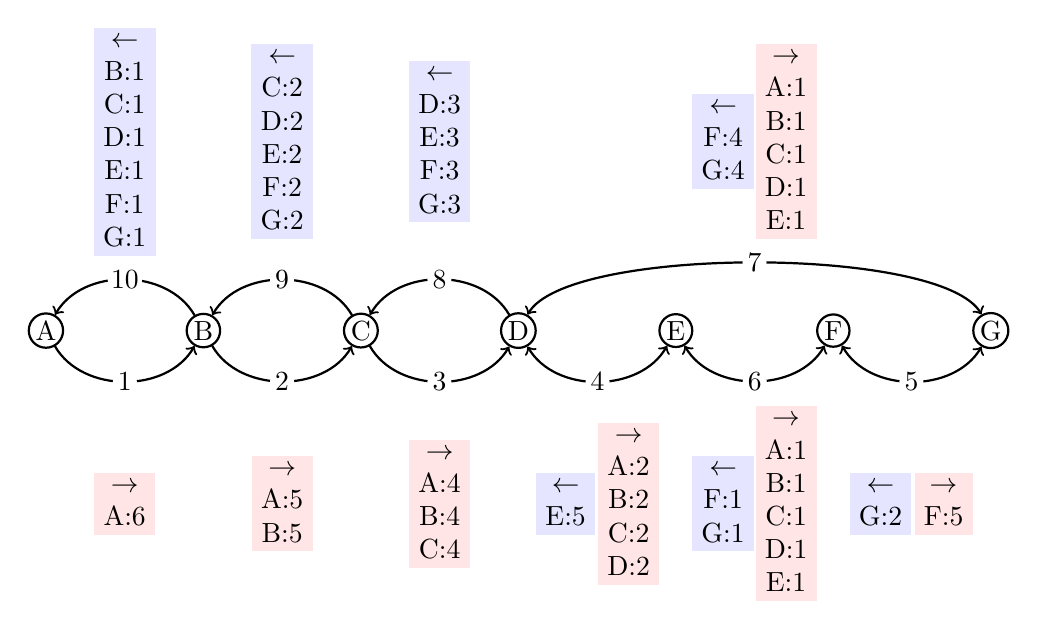
\begin{tikzpicture}[scale=2,thick,line cap=round]
	\tikzstyle{jiao}=[solid,circle,draw,fill=white,inner sep=.8pt];
	\tikzstyle{bian}=[circle,fill=white,inner sep=.2pt];
	% %% title
	% \node at (3,2.2) {How to share cookies between 7 people with the fewest swaps?};
	%% graph
	\node[jiao] (A) at (0,0) {A};
	\node[jiao] (B) at (1,0) {B};
	\node[jiao] (C) at (2,0) {C};
	\node[jiao] (D) at (3,0) {D};
	\node[jiao] (E) at (4,0) {E};
	\node[jiao] (F) at (5,0) {F};
	\node[jiao] (G) at (6,0) {G};
	\draw (A) edge[->,bend  right=60]               node[bian]{1}  (B);
	\draw (B) edge[->,bend  right=60]               node[bian]{2}  (C);
	\draw (C) edge[->,bend  right=60]               node[bian]{3}  (D);
	\draw (D) edge[<->,bend right=60]               node[bian]{4}  (E);
	\draw (E) edge[<->,bend right=60]               node[bian]{6}  (F);
	\draw (F) edge[<->,bend right=60]               node[bian]{5}  (G);
	\draw (G) edge[<->,bend right=60,looseness=.45] node[bian]{7}  (D);
	\draw (D) edge[->,bend  right=60]               node[bian]{8}  (C);
	\draw (C) edge[->,bend  right=60]               node[bian]{9}  (B);
	\draw (B) edge[->,bend  right=60]               node[bian]{10} (A);
	\begin{scope}[xshift=0.5cm,yshift=-1.1cm]
		\node[fill=red!10,align=center]  at (0,0)     {$\rightarrow$\\A:6};
		\node[fill=red!10,align=center]  at (1,0)     {$\rightarrow$\\A:5\\B:5};
		\node[fill=red!10,align=center]  at (2,0)     {$\rightarrow$\\A:4\\B:4\\C:4};
		\node[fill=red!10,align=center]  at (3+0.2,0) {$\rightarrow$\\A:2\\B:2\\C:2\\D:2};
		\node[fill=blue!10,align=center] at (3-0.2,0) {$\leftarrow$\\E:5};
		\node[fill=red!10,align=center]  at (5+0.2,0) {$\rightarrow$\\F:5};
		\node[fill=blue!10,align=center] at (5-0.2,0) {$\leftarrow$\\G:2};
		\node[fill=red!10,align=center]  at (4+0.2,0) {$\rightarrow$\\A:1\\B:1\\C:1\\D:1\\E:1};
		\node[fill=blue!10,align=center] at (4-0.2,0) {$\leftarrow$\\F:1\\G:1};
	\end{scope}
	\begin{scope}[xshift=0.5cm,yshift=1.2cm]
		\node[fill=red!10,align=center]  at (4+0.2,0) {$\rightarrow$\\A:1\\B:1\\C:1\\D:1\\E:1};
		\node[fill=blue!10,align=center] at (4-0.2,0) {$\leftarrow$\\F:4\\G:4};
		\node[fill=blue!10,align=center] at (2,0)     {$\leftarrow$\\D:3\\E:3\\F:3\\G:3};
		\node[fill=blue!10,align=center] at (1,0)     {$\leftarrow$\\C:2\\D:2\\E:2\\F:2\\G:2};
		\node[fill=blue!10,align=center] at (0,0)     {$\leftarrow$\\B:1\\C:1\\D:1\\E:1\\F:1\\G:1};
	\end{scope}
\end{tikzpicture}

\end{document}
